\chapter{Implementación y Despliegue del Software de Control}
\label{cha:software_control}

Este capítulo describe la arquitectura del software de control local, la lógica de las rutinas de control implementadas, su integración con la plataforma de telemetría en la nube ThingSpeak, y la interfaz de usuario del sistema.

\section{Código}
\label{sec:codigo}

\subsection{Sistema operativo y lenguaje de desarrollo}
\label{subsec:so_lenguaje}

El software de control se ejecuta sobre Raspberry Pi OS (anteriormente denominado Raspbian), la distribución oficial de Linux basada en Debian mantenida por la Raspberry Pi Foundation para las computadoras de placa única de esta familia. La elección de este sistema operativo no fue una decisión de diseño independiente, sino una consecuencia directa de la selección de la Raspberry Pi 4 Model B como unidad de procesamiento central (Sección \ref{sec:raspberry_pi}): al tratarse de la distribución de referencia del fabricante, garantiza la compatibilidad completa con los periféricos de hardware embebido (GPIO, bus I2C) a través de sus bibliotecas oficiales, sin requerir capas de compatibilidad adicionales.

Todo el software desarrollado --la lógica de adquisición y control, el registro de datos, la integración con la nube y la interfaz web de configuración-- se implementó íntegramente en Python. Esta elección aprovecha directamente las ventajas de concurrencia y gestión de librerías discutidas en la Sección \ref{sec:raspberry_pi}: Python cuenta con soporte oficial de primer nivel en Raspberry Pi OS, y dispone de bibliotecas maduras tanto para el acceso a hardware embebido (a través del proyecto Adafruit Blinka, que expone una capa de compatibilidad CircuitPython sobre los pines GPIO y el bus I2C de la Raspberry Pi) como para el desarrollo de servicios web (mediante el microframework Flask, utilizado para la interfaz de usuario de la Sección \ref{sec:interfaz_usuario}).

\subsection{Organización modular del software}
\label{subsec:organizacion_modular_real}

Siguiendo el principio de separación de responsabilidades presentado en el Marco Teórico (Sección \ref{sec:modularidad}), el software del prototipo se organiza en seis módulos de Python, cada uno responsable de un único bloque funcional:

\begin{itemize}
    \item \texttt{models.py}: define, mediante clases de datos (\textit{dataclasses}), la estructura de la configuración del sistema (\texttt{SystemConfig}, \texttt{MacetaConfig}, y las configuraciones anidadas de cada sensor y actuador) y la estructura del estado en tiempo de ejecución (\texttt{MacetaEstado}), sin contener ninguna lógica propia. Es la representación del estado descripta de forma genérica en el Marco Teórico.
    \item \texttt{config\_loader.py}: implementa la configuración externalizada (Sección \ref{subsec:config_externalizada_real}), leyendo el archivo de configuración y construyendo las estructuras de \texttt{models.py} a partir de él, además de validar su consistencia antes de iniciar el sistema.
    \item \texttt{hardware.py}: implementa la capa de abstracción de hardware (Sección \ref{subsec:capa_hardware_real}), traduciendo operaciones de alto nivel (``leer humedad de suelo'', ``encender luz'') a las operaciones concretas de bus I2C y de pines GPIO.
    \item \texttt{control.py}: contiene la lógica de control propiamente dicha --las funciones de decisión de riego, ventilación y DLI presentadas en el Capítulo \ref{cha:hardware_control}--, sin conocer ningún detalle de cómo se leen los sensores ni de cómo se accionan los actuadores.
    \item \texttt{main.py}: implementa la orquestación del sistema (Sección \ref{subsec:ciclo_orquestacion}): el ciclo principal que en cada iteración coordina la lectura de sensores, la invocación de la lógica de control, la actuación sobre el hardware, el registro persistente en CSV y el envío de telemetría a ThingSpeak.
    \item \texttt{web.py}: implementa la interfaz de salida de configuración remota (Sección \ref{sec:interfaz_usuario}), exponiendo un servidor web que permite consultar y modificar los parámetros del sistema sin necesidad de acceso directo a la Raspberry Pi.
\end{itemize}

Esta organización refleja de forma directa los seis bloques de separación de responsabilidades enumerados en el Marco Teórico: configuración (\texttt{config\_loader.py}), representación del estado (\texttt{models.py}), abstracción de hardware (\texttt{hardware.py}), lógica de control (\texttt{control.py}), orquestación (\texttt{main.py}) e interfaces de salida (\texttt{web.py}, junto con las rutinas de registro CSV y telemetría dentro de \texttt{main.py}).

La Figura \ref{fig:arquitectura_control} muestra las dependencias de importación reales entre los cuatro módulos que conforman el proceso de control (\texttt{indoor\_main.service}, Sección \ref{subsec:systemd}), junto con las funciones y clases principales que expone cada uno.

\begin{figure}[htbp]
\centering
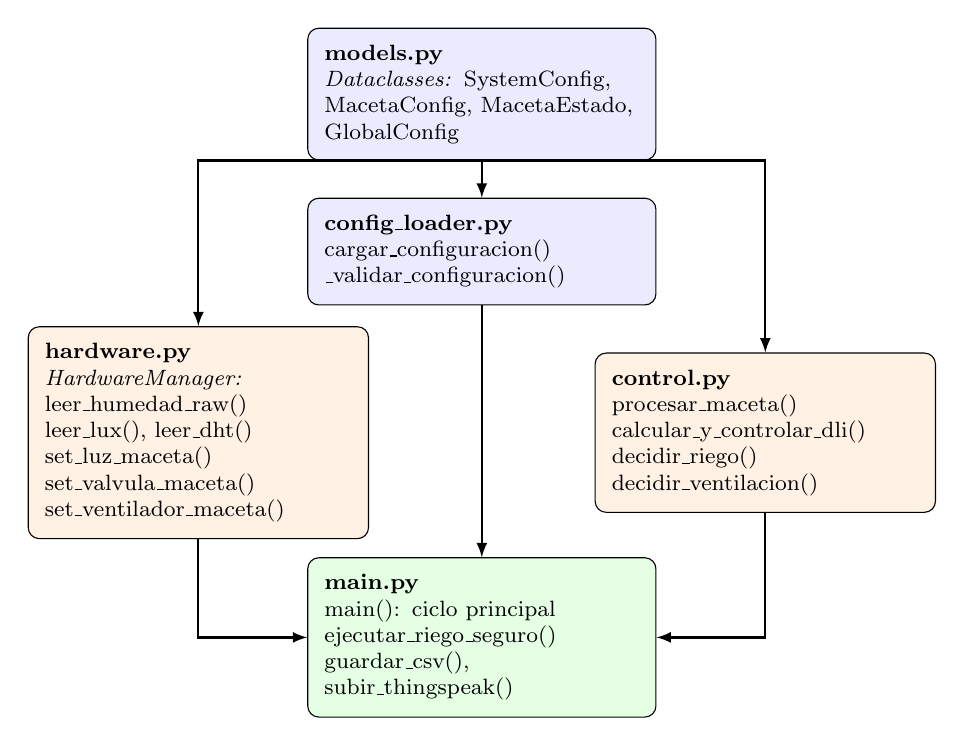
\begin{tikzpicture}[
    modulo/.style={rectangle, draw=black, rounded corners, align=left, font=\footnotesize, text width=4cm, inner sep=6pt},
    flujo/.style={-latex, thick},
]

\node (models) [modulo, fill=blue!8] at (3.6,7.2) {\textbf{models.py}\\ \textit{Dataclasses:} SystemConfig, MacetaConfig, MacetaEstado, GlobalConfig};

\node (configloader) [modulo, fill=blue!8] at (3.6,5.2) {\textbf{config\_loader.py}\\ cargar\_configuracion()\\ \_validar\_configuracion()};

\node (hardware) [modulo, fill=orange!10, text width=3.9cm] at (0,2.9) {\textbf{hardware.py}\\ \textit{HardwareManager:}\\ leer\_humedad\_raw()\\ leer\_lux(), leer\_dht()\\ set\_luz\_maceta()\\ set\_valvula\_maceta()\\ set\_ventilador\_maceta()};

\node (control) [modulo, fill=orange!10, text width=3.9cm] at (7.2,2.9) {\textbf{control.py}\\ procesar\_maceta()\\ calcular\_y\_controlar\_dli()\\ decidir\_riego()\\ decidir\_ventilacion()};

\node (main) [modulo, fill=green!10] at (3.6,0.3) {\textbf{main.py}\\ main(): ciclo principal\\ ejecutar\_riego\_seguro()\\ guardar\_csv(), subir\_thingspeak()};

\draw [flujo] (models) -- (configloader);
\draw [flujo] (models.south) -| (hardware.north);
\draw [flujo] (models.south) -| (control.north);
\draw [flujo] (configloader) -- (main);
\draw [flujo] (hardware) |- (main.west);
\draw [flujo] (control) |- (main.east);

\end{tikzpicture}
\caption{Dependencias de importación entre los módulos del proceso de control (\texttt{indoor\_main.service}). Todas las flechas representan relaciones de código (\textit{import}): \texttt{main.py} depende de los tres módulos restantes, que a su vez comparten las estructuras de datos definidas en \texttt{models.py}.}
\label{fig:arquitectura_control}
\end{figure}

Como contrapunto, la Figura \ref{fig:arquitectura_web} muestra que el proceso de configuración web (\texttt{indoor\_web.service}) --detallado en la Sección \ref{sec:interfaz_usuario}-- \textbf{no importa ni depende de ningún código} de los módulos anteriores: es un proceso de Python completamente independiente, que solo comparte con el proceso de control el archivo \texttt{config.toml} en disco. Esta ausencia deliberada de acoplamiento por código es consistente con la decisión de ejecutar ambos procesos como servicios de \texttt{systemd} separados y sin dependencias de arranque explícitas entre sí (Sección \ref{subsec:systemd}).

\begin{figure}[htbp]
\centering
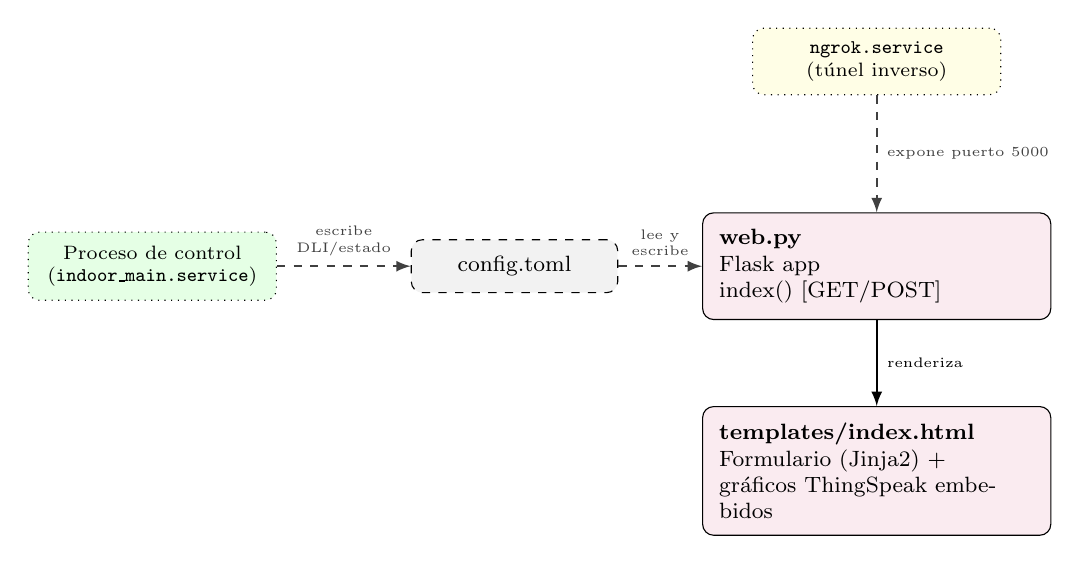
\begin{tikzpicture}[
    modulo/.style={rectangle, draw=black, rounded corners, align=left, font=\footnotesize, text width=4cm, inner sep=6pt},
    archivo/.style={rectangle, draw=black, dashed, rounded corners, align=center, font=\footnotesize, fill=gray!10, text width=2.2cm, inner sep=6pt},
    servicio/.style={rectangle, draw=black, dotted, rounded corners, align=center, font=\scriptsize, fill=yellow!10, text width=2.8cm, inner sep=5pt},
    flujoarch/.style={-latex, dashed, thick, gray!50!black},
    flujo/.style={-latex, thick},
]

\node (mainproc) [servicio, fill=green!10] at (-0.6,2.6) {Proceso de control\\ (\texttt{indoor\_main.service})};

\node (toml) [archivo] at (4.0,2.6) {config.toml};

\node (web) [modulo, fill=purple!8] at (8.6,2.6) {\textbf{web.py}\\ Flask app\\ index() [GET/POST]};

\node (ngrok) [servicio] at (8.6,5.2) {\texttt{ngrok.service}\\ (túnel inverso)};

\node (template) [modulo, fill=purple!8] at (8.6,0.0) {\textbf{templates/index.html}\\ Formulario (Jinja2) +\\ gráficos ThingSpeak embebidos};

\draw [flujoarch] (mainproc.east) -- node[above,font=\tiny,align=center]{escribe\\ DLI/estado} (toml.west);
\draw [flujoarch] (toml.east) -- node[above,font=\tiny,align=center]{lee y\\ escribe} (web.west);
\draw [flujoarch] (ngrok.south) -- node[right,font=\tiny]{expone puerto 5000} (web.north);
\draw [flujo] (web.south) -- node[right,font=\tiny]{renderiza} (template.north);

\end{tikzpicture}
\caption{Relación entre el proceso de control y el proceso de configuración web (\texttt{indoor\_web.service}). A diferencia de la Figura \ref{fig:arquitectura_control}, aquí no existe ninguna dependencia de código Python entre ambos procesos: la única relación es el archivo \texttt{config.toml} compartido en disco (flechas punteadas), que cada proceso lee y/o escribe de forma independiente. El servicio \texttt{ngrok.service} tampoco depende del código de \texttt{web.py}; únicamente reenvía tráfico de red hacia el puerto que este último expone.}
\label{fig:arquitectura_web}
\end{figure}

\subsection{Configuración externalizada}
\label{subsec:config_externalizada_real}

Todos los parámetros ajustables del sistema --umbrales de control, factores de luminaria, direcciones I2C, asignación de pines GPIO, credenciales de ThingSpeak, entre otros-- se externalizan en un único archivo de configuración en formato TOML (\texttt{config.toml}), aplicando directamente el patrón de configuración externalizada descripto en el Marco Teórico (Sección \ref{sec:config_persistencia}). A modo ilustrativo, la configuración de una maceta incluye:

\begin{verbatim}
[macetas.maceta1]
umbral_humedad_suelo_raw = 150
umbral_humedad_ambiente_pct = 80.0
umbral_temperatura_c = 30
tiempo_riego_seg = 60.0
hora_inicio_dia = 10
hora_fin_dia = 22
dli_objetivo = 15.0
lux_foco = 6500
factor_luminaria = 0.0887
factor_luminaria_ambiente = 0.0185
\end{verbatim}

El módulo \texttt{config\_loader.py} no se limita a parsear este archivo: antes de que el sistema comience a operar, ejecuta un conjunto de validaciones de consistencia sobre la configuración cargada, entre ellas: que los umbrales porcentuales se encuentren dentro del rango físicamente válido (0 a 100), que no existan direcciones I2C repetidas entre distintos conversores A/D, y que no haya dos actuadores o sensores distintos asignados al mismo pin GPIO. Esta validación temprana evita que un error de tipeo en el archivo de configuración --por ejemplo, dos actuadores compartiendo accidentalmente el mismo GPIO-- se manifieste recién en tiempo de ejecución como una falla de hardware difícil de diagnosticar.

\subsection{Capa de abstracción de hardware}
\label{subsec:capa_hardware_real}

La clase \texttt{HardwareManager} centraliza todo el acceso físico a sensores y actuadores, exponiendo hacia el resto del sistema métodos de alto nivel (\texttt{leer\_humedad\_raw}, \texttt{leer\_lux}, \texttt{leer\_dht}, \texttt{set\_luz\_maceta}, \texttt{set\_valvula\_maceta}, \texttt{set\_ventilador\_maceta}, entre otros) que ocultan por completo los detalles de bus I2C y de numeración de pines GPIO al módulo de control. Dos aspectos de su implementación aplican directamente principios ya presentados en el Marco Teórico:

En primer lugar, la lectura de humedad de sustrato (\texttt{leer\_humedad\_raw}) toma una primera lectura de descarte antes de comenzar el muestreo real, y luego promedia 5 lecturas sucesivas del conversor A/D. La lectura de descarte responde directamente al comportamiento del PCF8591 descripto en el Marco Teórico (Sección \ref{subsec:conversion_ad}): tras una condición de reinicio, o al cambiar de canal, el primer byte transmitido corresponde a una conversión anterior y no al canal actualmente seleccionado, por lo que se descarta explícitamente antes de tomar las muestras válidas. El promedio de las 5 lecturas posteriores implementa, a nivel de hardware, el sobremuestreo (\textit{oversampling}) también presentado en esa misma sección.

En segundo lugar, la configuración de cada pin de salida (\texttt{\_configurar\_salida}) fija el nivel lógico seguro del actuador \textit{antes} de conmutar el pin al modo salida, evitando así un pulso espurio de activación en el instante en que el microcontrolador toma control del pin --una precaución directamente relacionada con la lógica de activación por nivel bajo descripta en el Marco Teórico (Sección \ref{subsec:activo_bajo}), dado que un pin flotante o mal inicializado podría interpretarse transitoriamente como un nivel bajo y disparar el relé de forma no intencional durante el arranque del sistema.

\subsection{Ciclo principal de orquestación}
\label{subsec:ciclo_orquestacion}

El módulo \texttt{main.py} ejecuta un ciclo continuo que, en cada iteración, repite la siguiente secuencia para cada maceta habilitada: lectura de sensores a través de \texttt{hardware.py}, procesamiento de esas lecturas mediante \texttt{control.py} (Capítulo \ref{cha:hardware_control}), y aplicación del nuevo estado resultante sobre los actuadores de luz y ventilación. A diferencia de un ciclo de control de período fijo, el intervalo real transcurrido entre iteraciones ($\Delta t$) se mide explícitamente en cada vuelta del ciclo, y es ese valor medido --no un valor nominal supuesto-- el que se utiliza para la integración del DLI (Ecuación \ref{eq:dli_ppfd} del Marco Teórico), evitando que una eventual demora en el ciclo de lectura introduzca un error sistemático en la acumulación diaria de luz. El acumulador de DLI, además, se reinicia automáticamente a cero al detectar un cambio de día calendario.

El riego se gestiona de forma diferenciada del resto de los actuadores, mediante una rutina de ejecución segura (\texttt{ejecutar\_riego\_seguro}) que introduce una secuencia de enclavamiento explícita para evitar condiciones de riego simultáneo entre macetas --consistente con la disposición física de una única bomba y línea compartida descripta en la Sección \ref{sec:circuito_riego}--:

\begin{enumerate}
    \item Un indicador global de exclusión mutua impide que se inicie un nuevo riego mientras otro ya está en curso; si el sistema está ocupado, el pedido de riego de esa maceta queda pendiente para el siguiente ciclo.
    \item Como medida preventiva, se cierran explícitamente las válvulas de todas las macetas antes de abrir la correspondiente a la maceta objetivo, evitando que un estado inconsistente previo deje dos válvulas abiertas a la vez.
    \item Se abre la válvula de la maceta objetivo y se introduce una breve espera antes de encender la bomba, asegurando que el camino hidráulico ya esté disponible en el momento en que comienza a circular agua a presión.
    \item Transcurrido el tiempo de riego configurado, la bomba se apaga \textit{antes} que la válvula, y se introduce una segunda espera (el tiempo de despresurización configurado) antes de cerrar la válvula, evitando que la manguera quede presurizada tras el cierre.
\end{enumerate}

Esta secuencia se ejecuta dentro de un bloque de manejo de excepciones que garantiza el apagado de la bomba y el cierre de la válvula --y la liberación del indicador de exclusión mutua-- incluso si ocurriera un error durante el riego, evitando que una falla de software derive en una válvula o una bomba que permanezcan indefinidamente activas.

Al finalizar el procesamiento de todas las macetas en cada ciclo, el sistema registra el estado completo en el archivo CSV local (Sección \ref{subsubsec:adquisicion_registro}) y transmite las variables relevantes a ThingSpeak (Sección \ref{subsec:thingspeak}), antes de aguardar el intervalo de lectura configurado e iniciar el siguiente ciclo. Ante una interrupción del programa --ya sea manual o por una excepción no controlada--, un bloque de finalización garantizado apaga todos los actuadores y libera los recursos de GPIO utilizados, evitando dejar relés activados tras la detención del sistema.

\subsection{Despliegue y arranque automático: gestión mediante servicios de systemd}
\label{subsec:systemd}

Para garantizar que el sistema comience a operar de forma autónoma inmediatamente después de energizar la Raspberry Pi --sin requerir que un operador inicie manualmente ningún proceso--, los tres componentes de software que deben ejecutarse de forma continua (el ciclo de control principal, el servidor web de configuración, y el túnel inverso de acceso remoto) se gestionan como servicios del sistema mediante \texttt{systemd}, el gestor de servicios estándar de Raspberry Pi OS.

Se definieron tres unidades de servicio independientes: \texttt{indoor\_main.service} (ejecuta el ciclo de orquestación de \texttt{main.py}, Sección \ref{subsec:ciclo_orquestacion}), \texttt{indoor\_web.service} (ejecuta el servidor Flask de \texttt{web.py}, Sección \ref{sec:interfaz_usuario}) y \texttt{ngrok.service} (ejecuta el túnel inverso presentado en el Marco Teórico, Sección \ref{sec:tunel_inverso}). Las tres unidades comparten la misma estructura de configuración:

\begin{itemize}
    \item \texttt{After=network.target}: cada servicio espera a que la interfaz de red del sistema esté disponible antes de iniciar su ejecución. Esto es particularmente relevante para \texttt{indoor\_main.service} (que depende de la red para la telemetría hacia ThingSpeak) y para \texttt{ngrok.service} (cuyo propósito es, precisamente, establecer una conexión de red saliente), evitando que intenten operar sobre una interfaz de red todavía no inicializada durante el arranque del sistema.
    \item \texttt{Restart=always}: ante la finalización inesperada de cualquiera de los tres procesos --por ejemplo, por una excepción no controlada--, \texttt{systemd} lo reinicia automáticamente sin intervención humana. Esta política de reinicio automático es la que materializa, a nivel de infraestructura de despliegue, el requisito de operación autónoma de la capa de procesamiento local planteado en el Marco Teórico (Sección \ref{sec:arquitectura_capas}).
    \item \texttt{WantedBy=multi-user.target}: habilita el arranque automático de los tres servicios durante el proceso de inicio del sistema operativo, sin requerir que un usuario inicie sesión ni ejecute manualmente ningún comando.
\end{itemize}

Los tres servicios se ejecutan como procesos independientes, sin una relación de dependencia u orden de arranque explícito entre ellos --ninguno declara al otro como requisito previo--. Esta independencia es intencional: el servidor de configuración web y el túnel de acceso remoto no requieren que el ciclo de control esté corriendo para cumplir su función (permitir la consulta y edición de la configuración, y exponer el puerto del servidor web hacia internet, respectivamente), por lo que acoplar su arranque al del proceso de control introduciría una dependencia innecesaria. Como contrapartida, no existe una garantía explícita de que \texttt{ngrok.service} inicie después de que \texttt{indoor\_web.service} ya esté escuchando en su puerto; en la práctica esto no representa un problema operativo relevante, dado que la política \texttt{Restart=always} y el propio comportamiento de reconexión de ngrok absorben cualquier intento de conexión fallido en los primeros segundos posteriores al arranque.
\subsubsection{Adquisición de Datos y Registro Histórico del Sistema}
\label{subsubsec:adquisicion_registro}

Para la persistencia, estructuración y posterior análisis de las variables físicas recopiladas durante las campañas de ensayo, el sistema implementa la generación automática de archivos con formato de valores separados por comas. Este estándar abierto de texto plano almacena la información tabulada en filas y columnas mediante delimitadores, consolidando en cada registro una estampa temporal (timestamp) de alta resolución que integra de forma simultánea tanto las lecturas de los sensores como el estado operativo de los actuadores. Por un lado, se registran las variables de entrada procesadas por la red de captación (incluyendo parámetros microclimáticos como la temperatura ambiente, la humedad relativa, la iluminancia en luxes, el DLI acumulado y la humedad volumétrica del sustrato en ambas macetas). Por otro lado, se almacenan las variables lógicas binarias que representan la activación o desactivación de los elementos de control, tales como los módulos de iluminación artificial y las bombas de riego. La elección del formato .csv se fundamenta en su baja carga computacional, su eficiencia en el consumo de memoria en el microcontrolador y su elevada interoperabilidad, lo que permite importar e integrar el dataset histórico de manera directa en entornos de procesamiento como Python para la posterior reconstrucción y análisis estadístico del comportamiento del prototipo.

\subsection{Telemetría y visualización en la nube: integración con ThingSpeak}
\label{subsec:thingspeak}

Para dotar al sistema de capacidades de monitoreo remoto propias del Internet de las Cosas (IoT), se implementó la plataforma en la nube ThingSpeak. Desarrollada por MathWorks, esta herramienta permite la agregación, visualización y análisis de flujos de datos en tiempo real.

La elección de esta plataforma para el prototipo se fundamenta en múltiples ventajas operativas. En primer lugar, ofrece un nivel de uso gratuito y de libre acceso para proyectos académicos y de investigación, lo que elimina los costos de licenciamiento o alquiler de servidores privados. En segundo lugar, descentraliza la visualización de los datos; al enviar las lecturas críticas del entorno radicular y ambiental a la nube, el usuario adquiere la capacidad de auditar el estado del cultivo (humedad de suelo, iluminancia, temperatura y humedad relativa) desde cualquier dispositivo con acceso a Internet, independizándose de la red de área local donde opera el sistema. Esta arquitectura sienta las bases prácticas para la interconexión de múltiples granjas inteligentes en un futuro.

\subsubsection{Arquitectura de transmisión de datos}

El envío de la información hacia los servidores en la nube se ejecuta de manera cíclica en cada iteración del lazo de control principal del sistema. Para garantizar una comunicación eficiente y segura, el algoritmo de telemetría se estructuró en las siguientes etapas conceptuales:

\begin{itemize}
    \item \textbf{Autenticación y acondicionamiento:} El proceso inicia con la validación de credenciales mediante una clave de interfaz (API Key) única, la cual autoriza a la placa central a publicar información en su respectivo canal. Previo a la conformación del paquete de datos, las lecturas de los sensores sufren un proceso de acondicionamiento digital; los valores decimales son truncados para eliminar fluctuaciones minúsculas no representativas, optimizando así el ancho de banda y el peso de la trama de red enviada.
    \item \textbf{Tolerancia a fallos y operación local:} El aspecto más crítico de la rutina de transmisión es su diseño orientado a la robustez. La comunicación con los servidores externos incorpora mecanismos de seguridad como la limitación del tiempo máximo de espera (\textit{timeout}) y el manejo seguro de excepciones ante caídas de conexión.
    \item \textbf{Prioridad de control:} Estas medidas garantizan que, ante una eventual pérdida de acceso a Internet o latencia en los servidores remotos, el software no colapse ni detenga su ejecución. De este modo, la unidad central prioriza el control local, pudiendo continuar ininterrumpidamente con tareas críticas como la desactivación de la bomba de riego o el encendido de la iluminación, asegurando la integridad del cultivo sin importar el estado de las telecomunicaciones.
\end{itemize}

\PENDIENTE{agregar fotos de la plataforma ThingSpeak (canal, gráficos)}

\section{Interfaz de usuario}
\label{sec:interfaz_usuario}

La interfaz de usuario se implementó como una aplicación web mínima construida con Flask, aplicando directamente el patrón cliente-servidor descripto en el Marco Teórico (Sección \ref{sec:cliente_servidor}): el servidor --ejecutado localmente en la Raspberry Pi y expuesto remotamente mediante el túnel inverso presentado en la Sección \ref{sec:tunel_inverso}-- concentra el acceso de lectura y escritura al archivo de configuración, mientras que cualquier navegador web actúa como cliente, sin necesidad de tener instalada ninguna dependencia del proyecto.

La aplicación expone una única ruta que responde a dos métodos HTTP distintos. Ante una solicitud \texttt{GET}, el servidor lee el archivo de configuración vigente y renderiza una página que muestra los valores actuales de los parámetros editables de cada maceta. Ante una solicitud \texttt{POST} --generada al enviar el formulario de la página--, el servidor toma los nuevos valores ingresados, actualiza la estructura de configuración en memoria y la vuelve a escribir por completo sobre el archivo de configuración, sobrescribiendo la versión anterior. Los parámetros expuestos para edición remota por maceta son el umbral de humedad de sustrato, el umbral de humedad ambiente, el tiempo de riego y el DLI objetivo --es decir, precisamente los parámetros de umbral y calibración discutidos en el Capítulo \ref{cha:hardware_control}--, mientras que el resto de la configuración (asignación de pines, direcciones I2C, credenciales de ThingSpeak) permanece fija y solo es editable directamente sobre el archivo.

Es importante remarcar que el código Python de \texttt{web.py} (Sección \ref{subsec:organizacion_modular_real}) resuelve únicamente la lectura y escritura del archivo de configuración y el enrutamiento HTTP; la estructura visual de la página --el formulario, sus etiquetas y estilos-- está definida por completo en un archivo de plantilla HTML separado (\texttt{templates/index.html}), siguiendo el patrón de plantillas de Flask basado en el motor Jinja2. Cada campo del formulario se vincula, mediante su atributo \texttt{name}, directamente con una clave del archivo de configuración: por ejemplo, el campo correspondiente al umbral de riego de la maceta 1 se declara en el HTML con \texttt{name="m1\_suelo"}, y es precisamente esa cadena la que \texttt{web.py} utiliza para leer el valor enviado y asignarlo a \texttt{config['macetas']['maceta1']['umbral\_humedad\_suelo\_raw']} antes de reescribir el archivo TOML. De manera análoga, cada campo se inicializa con el valor vigente en la configuración mediante una expresión de plantilla Jinja2 (por ejemplo, \texttt{\{\{ config.macetas.maceta1.umbral\_humedad\_suelo\_raw \}\}}), de modo que la página siempre refleja el estado real del archivo al momento de cargarse, y no un valor por defecto codificado en el HTML.

Más allá del formulario de configuración, la misma página incorpora una sección de monitoreo histórico que embebe directamente, mediante elementos \texttt{iframe}, los gráficos públicos generados por la plataforma ThingSpeak (Sección \ref{subsec:thingspeak}) para cada campo de cada canal. De esta forma, la interfaz cumple una doble función en una única página: permite tanto la edición remota de los parámetros de control como la visualización de la evolución histórica de las variables de cada maceta, sin necesidad de que el usuario abandone la página ni de que el propio servidor Flask genere ningún gráfico por su cuenta --esa tarea queda completamente delegada a ThingSpeak--. Cabe destacar que toda la interfaz se resuelve mediante renderizado del lado del servidor: no se emplea código JavaScript propio ni actualización asincrónica de datos, por lo que cada cambio de valores requiere un envío de formulario y una recarga completa de la página, una decisión de diseño consistente con el criterio general de simplicidad y bajo costo de mantenimiento adoptado en el resto del proyecto.

Tras procesar una solicitud de guardado exitosa, el servidor redirige al usuario nuevamente a la página principal en lugar de responder directamente sobre la misma solicitud POST, evitando así que una recarga accidental de la página por parte del usuario reenvíe el mismo formulario y sobrescriba la configuración por segunda vez. Esta misma respuesta de redirección incluye una señal que la página utiliza para mostrar una confirmación visual de que los cambios se guardaron correctamente.

\PENDIENTE{agregar fotos/capturas de pantalla de la interfaz web}
